\chapter{Zusammenfassung und Ausblick}
\label{Zusammenfassung}

\section{Zusammenfassung und Ausblick}

In dieser Arbeit war es das Ziel eine Datenbankanwendung zu implementieren, die auf SQL-Anfragen hin, Index-basierte Antworten liefert. \\
Es ist möglich über den Client verschiedene SQL-Statements an den Server, bzw. die Datenbankanwendung, zu senden und diese mithilfe der verschiedenen Services auswerten zu lassen. 
Diese Services basieren auf Apache Arrow und Gandiva. Apache Arrow zum einpflegen der Daten in den Hauptspeicher in einem spezifischen und performanten Spalten-Format und Gandiva zum Auswerten dieser Daten, mithilfe von Filtern. 
Die Datenbankanwendung interpretiert eigenständig verschiedene Arten von SQL-Statements. Jedoch konnten nicht alle Arten von Statements in dieser Arbeit umgesetzt werden. 
Es wurde jedoch in Abschnitt \ref{erweitern} erläutert, inwiefern diese erweitert werden können.

In \ref{Einleitung} wurde auf den Non Volatile Ram eingegangen, der für die Arbeit ein wichtiger Ausblick ist. 
Sobald Apache Arrow mit Non Volatile Ram kompatibel ist, wäre es möglich den Zustand der Datenbankanwendung bei dem erneuten Starten der Maschine, sofort ohne Initialisierung, zurück zu erhalten. Dies würde die Performance der Index-basierten Datenbankanwendung  steigern und es könnten Energieersparnisse deutlich gemacht werden.
\\
Verschiedene Operationen, wie die Summierung von Spalten, die zu einer genaueren Analyse der Performance der Datenbankanwendung hilfreich wären, oder die Initialisierung von mehreren Tables, konnten nicht mit in diese Arbeit einfließen, da diese den Arbeitsumfang deutlich überschreiten würden. Jedoch ist es notwendig zu erwähnen, dass durch das Framework Apache Arrow eine solide Basis zur Speicherung von großen Datenmengen im Hauptspeicher geschaffen wurde.
Mit dem Hintergedanken, dass nicht das ganze Datenset, sondern nur die Speicheradressen mit verschiedenen Offsets, auf Anfrage hin ,zurückgeliefert werden, entstehen neue Möglichkeiten in der Datenbankverwaltung.
\\ 
Mit Hinblick auf die Technologie Remote Direct Memory Access, ist es denkbar, dass ein Vorteil dadurch entsteht, dass die Anfrage von Daten, keine große Datenmenge mehr über die Verbindung vom Server zum Client schickt, sondern diese Übertragung von relevanten, angefragten Daten ausgelagert wird.

\begin{figure}[h]
  \centering
  \begin{subfigure}[b]{0.5\textwidth}
    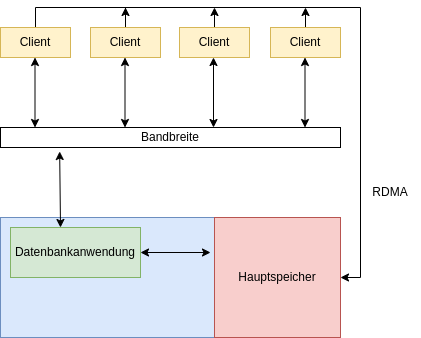
\includegraphics[width=1.0\linewidth]{img/rdma}
  \end{subfigure}
  \caption{Remote Direct Memory Access Schema mit Datenbankanwendung}
  \label{graf6}
\end{figure}

Somit können mehrere Clients im Netzwerk große Anfragen an die Datenbankanwendung schicken und sich danach selbst, um das Besorgen der Daten kümmern. Die Datenbankanwendung liefert nur noch die Speicher-Adressen und Offsets, bzw. Indices und keine großen Datenmengen mehr über die Verbindung zurück. In der Grafik \ref{graf6} wurde solch ein Fall zum besseren Verständnis visualisiert.







